\chapter{Mathematical Modeling Basics}

\section{A general class of models}
The class of models we will be concerned about takes this form;
\begin{equation}
    \dot{x}_i(t) = x_i(t)\cdot f_i[x(t)]
\end{equation}
The reason behind the choice to factor out $x_i$ is to highlight that in this class of models invasion of the ecosystem is not allowed: if a species is not present at time $t=0$, it cannot enter the ecosystem at later times. 
\section{Types of ecological interactions, with some real world examples}
\begin{figure}[H]
\centering
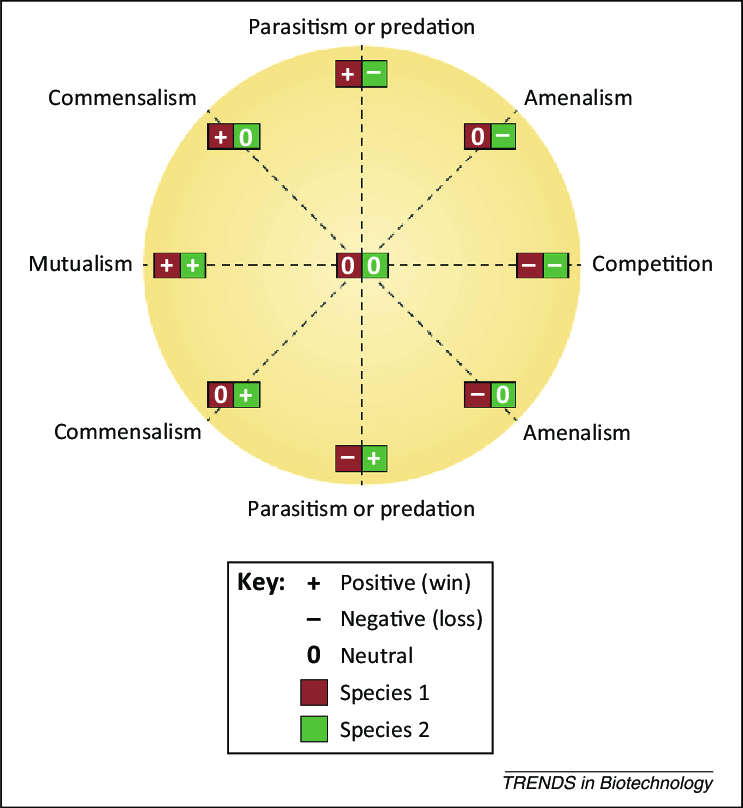
\includegraphics[width=0.4\linewidth]{figures/chapter_1/Ecological-interactions-among-microbial-species-For-any-two-interacting-species-there.png}
    \caption{The six types of ecological interactions}
    \label{fig:eco_interactions}
\end{figure}
\begin{itemize}
    \item Syntrophy: is a specific type of mutualistic (+ +) relationship where two or more species cooperate to degrade a substrate that neither species can break down alone. The metabolic products of one organism are essential for the other organism to thrive, and vice versa. Syntrophy often occurs when the degradation of a compound requires a sequential or coupled process that depends on the interaction of different species.
	The classic example is methanogenic syntrophy in anaerobic environments: certain bacteria break down complex organic matter into simpler compounds like hydrogen ($H_2$) and acetate. However, high levels of $H_2$ can inhibit their activity. Methanogens (archaea) consume $H_2$, converting it into methane ($CH_4$), which lowers the $H_2$ concentration, allowing the bacteria to continue their breakdown process. Without the methanogens, the bacteria couldn’t degrade the organic matter efficiently. This makes the interaction beneficial for both sides (++). 
	\item Cross-Feeding: is a broader term that refers to any process where one organism consumes the metabolic by-products of another organism, regardless of whether this interaction is obligatory for either species. It can be mutualistic (+ +), but it can also be commensal (+ 0), where one species benefits without affecting the other. A well-known example is lactate cross-feeding in the human gut microbiome: \textit{Bifidobacteria} ferment dietary fibers into lactate. Certain butyrate-producing bacteria, such as \textit{Eubacterium hallii}, consume lactate and convert it into butyrate, a short-chain fatty acid beneficial for gut health. This relationship benefits the butyrate producers but is not strictly required for the bifidobacteria.
\end{itemize}
\section{Ecological interactions can be context- dependent}
There is experimental evidence that the type  (the sign) and the strength of ecological interactions between species can change, depending on biotic and abiotic \footnote{Biotic means living and abiotic means non - living. For example, considering the microbiota ecosystem, some abiotic factors include the host's diet, the host's immune system response, the body temperature. Biotic factors, instead, include for example the metabolic products of the species and the species population densities.} factors in the environment. This fact is commonly referred to as \textit{context-dependency}. That is, there are situations where the type of interaction (mutualism, commensalism, competition etc..) cannot be assumed as fixed, and species can behave in different ways with respect to each other if conditions change in the environment, for example switching from midly competing to strongly competing, or even from competing to mutualistic and so on.

In mathematical terms, this means that the sign pattern of the Jacobian matrix at equilibrium (the community matrix) may change across the different steady (or equilibrium) states of the system. The community matrix details the effect of increasing the density of one species on any other species around the equilibrium point.


\begin{center}
\begin{align}
    \dot{x}_i(t) = x_i(t)\cdot f_i[x(t)] \\
    \overline{x}\,\, \text{steady state}\,\, J(\overline{x})_{i,\,j} = \frac{\partial f_i}{\partial_j} \,\, \text{community matrix at equilibrium}\,\, \overline{x}
\end{align}
\end{center}
This fact adds complexity to the task of building models for species evolution. 

\textbf{Key Idea}
   \textit{Species populations across different environmental conditions or community memberships generate distinct interspecies interaction networks, the comparison of which may provide an idea of how interactions are modulated by the impact of abiotic and biotic factors (es: how will the climate change affect the ecosystems?)} 

The generalized Lokta Volterra model does not account for context- dependency of interactions. Instead, one class of models that can account for context-dependency is the \textbf{Consumer - Resource models (CRM)} class. A paradigmatic CRM is the Mac Arthur's consumer-resource model (MCRM).

A general consumer-resource model consists of \( M \) resources whose abundances are \( R_1, \ldots, R_M \) and \( S \) consumer species whose populations are \( N_1, \ldots, N_S \). A general consumer-resource model is described by the system of coupled ordinary differential equations,

\[
\frac{dN_i}{dt} = N_i g_i(R_1, \ldots, R_M), \quad i = 1, \ldots, S,
\]

\[
\frac{dR_\alpha}{dt} = f_\alpha(R_1, \ldots, R_M, N_1, \ldots, N_S), \quad \alpha = 1, \ldots, M,
\]

where \( g_i \), depending only on resource abundances, is the per-capita growth rate of species \( i \), and \( f_\alpha \) is the growth rate of resource \( \alpha \). An essential feature of CRMs is that species growth rates and populations are mediated through resources and there are no explicit species-species interactions. Through resource interactions, there are emergent inter-species interactions.(source: Wikipedia Eng Consumer-Resource Models).




\subsection{Some real world examples of context - dependency}
Some of the most common factors that may shift the interaction type and strength are resource availability and population density.
\begin{itemize}
    \item Plant-fungi relationships (mutualism to commensalism to parasitism):

Many plants form mycorrhizal associations with fungi, where fungi enhance nutrient uptake for the plant (a mutualistic relationship). However, in nutrient-rich soils, allocating resources to the fungi can become disadvantageous for the plant. Thus, the fungi effectively becomes a parasite. \parencite{mycorrhizal}.

    \item Quorum sensing virulence expression:\\
    Bacteria often communicate using quorum sensing, a mechanism where they release signaling molecules into their environment to detect population density.  Many pathogenic bacteria are harmless when their population densities are low. At low densities, they might exist in a commensal relationship with the host or other bacteria. However, when their density surpasses a certain threshold (as detected via quorum sensing), they might collectively express virulence factors, turning from harmless commensals into aggressive pathogens.
    \item 
    Glucose alters the symbiotic relationships between the host and the gut microbiota. \\ For instance, glucose metabolism by Escherichia coli increases the production of organic acids,
    which lowers intestinal pH resulting in reduced survival of Vibrio cholerae in the
    host. This represents a mutualistic interaction between host glucose and a commensal
    (E. coli) to combat a potential pathogen (V.
    cholerae). Also, high glucose availability in the
    jejunum, cecum, and colon can result in
    increased glucose metabolism by certain
    pathogenic bacteria. This increased bacterial
    glucose flux can reduce virulence and tip the
    balance from parasitism to commensalism. 
    \parencite{doi:10.1152/ajpendo.00485.2019}.
\end{itemize}



\subsection{Community matrix in the gLV model has fixed sign pattern for feasible equilibria.}
The classic generalized lokta volterra is the simplest possible model of species interactions. It assumes fixed sign and strength of interactions. As a consequence of this assumption, \textit{the sign pattern of the community matrix is fixed across all feasible equilibria} \parencite{Allesina_Brasil}.

Generalized deterministic Lokta Volterra
\begin{equation}
    \centering
     \dot{x}_i(t) = x_i(t)\cdot \left[ r_i\, + \sum_j\, a_{i,\,j}\, x_j \right] \label{eq:gLV}
\end{equation}
where the $r_i$ are the intrinsic growth rates, $a_{i,\,j }$ are the interaction terms. Usually, growth rates are taken as negative to account for a limited carrying capacity of the environment (logistic growth).
In compact matrix form:
\begin{equation}
    \centering
    \dot{x} = \text{diag}(x)\,\cdot \left[r + A\cdot x\right] = f(x)
\end{equation}

Then lets compute the entries of the community matrix at the feasible equilibrium $\overline{x}$:
\begin{align}
    \begin{cases}
    \frac{\partial f_i}{\partial x_j} = a_{i,\,j}\, \overline{x}_i \quad i\neq j \\
    \frac{\partial f_i}{\partial x_j} = [r + A\overline{x}]_i+ a_{i,\,i}\overline{x}_i \quad i= j \\
    \end{cases}
\end{align}:
A \textit{feasible equilibrium}, by definition, is an equilibrium in the positive open subset of $\mathbb{R}^n$, $\mathbb{R}^n_{+} = \{x | x_i > 0\, \forall i\}$, that is an equilibrium where all the species coexist with positive abundances. Since in a feasible equilibrium $\text{diag}(\overline{x})$ has all positive entries, $\overline{x}$ must satisfy
\begin{equation}
\begin{cases}
r + A \overline{x} = 0 \\
\overline{x}_i > 0\quad \forall i \\
\end{cases}
\end{equation}
Solutions to the first equation depends on $rk[A|r]$.  Let us suppose solutions exist ($rk[A|r] = rk[A]$). The community matrix at the feasible equilibrium satisfies
\begin{equation}
    J_{i,\,j} = a_{i,\,j}\,\overline{x}_i \quad \forall x_{i,\,j}
\end{equation}
In particular, in case multiple feasible equilibria do exist ($rk[A]< n$ and $rk[A|r] = rk[A]$), the sign patter of their community matrix is always the same and is equal to the sign pattern of the interaction matrix $A$.
